\chapter{Design and Architecture}

\section*{Introduction to Chapter 4}
\addcontentsline{toc}{section}{Introduction to Chapter 4}

This chapter presents the design and architecture of the Intelligent Avionics Health Monitoring and Predictive Maintenance Platform. It is divided into two main parts. The first part describes the UAV conceptual design, including the selection of the UAV platform, propulsion system, and sensing strategy. The second part presents the software architecture, including the global system design, component architecture, database design, authentication strategy, and deployment architecture. The design decisions presented in this chapter establish the foundation for the implementation phases described in subsequent chapters.

\section{UAV Conceptual Design}

\subsection{UAV Type Selection and Justification}

The selection of the UAV platform is a critical design decision that influences the entire system architecture. Three main UAV categories were evaluated: fixed-wing aircraft, multi-rotor helicopters, and hybrid configurations. Fixed-wing UAVs were selected for this project for several reasons. First, fixed-wing aircraft offer superior flight endurance compared to rotary-wing platforms, which is essential for long-duration surveillance and inspection missions. Second, fixed-wing UAVs align with AVIONAV's product portfolio, specifically the U Storm large unmanned aerial vehicle designed for surveillance and inspection missions. Third, the linear flight profile of fixed-wing aircraft provides more stable telemetry data patterns, which simplifies the machine learning anomaly detection task. Multi-rotor platforms were rejected due to their limited battery life and highly variable power consumption patterns that would complicate anomaly detection. Hybrid configurations were rejected due to increased mechanical complexity, which would introduce additional failure modes beyond the scope of this project.

\subsection{Fixed-Wing UAV Description}

A Blended Wing Body (BWB) configuration with a rear-mounted pusher motor was selected as the UAV platform. This advanced aerodynamic configuration offers significant advantages for avionics health monitoring. The thick central fuselage pod provides a large internal volume to house the intelligent monitoring platform, flight controller, and batteries, ensuring adequate space for the monitoring electronics. The elimination of the traditional tail assembly reduces drag and structural weight, increasing flight endurance and simplifying the mechanical design. The rear-mounted pusher configuration places the propulsion system in a clean airflow region, reducing vibration and improving the quality of telemetry data. The swept wing geometry provides aerodynamic efficiency at cruise speeds while maintaining stability during surveillance operations.

\begin{figure}[H]
\centering
% 
\includegraphics[width=0.8\textwidth]{assets/figures/chapter4/fig_bwb_isometric.png}
\fbox{\parbox[c][4cm][c]{0.6\textwidth}{\centering Figure: Isometric view of the selected Blended Wing Body UAV platform}}
\caption{Isometric view of the selected Blended Wing Body UAV platform.}
\label{fig:uav_isometric}
\end{figure}

\begin{figure}[H]
\centering
% 
\includegraphics[width=0.8\textwidth]{assets/figures/chapter4/fig_bwb_top_view.png}
\fbox{\parbox[c][4cm][c]{0.6\textwidth}{\centering Figure: Top view of the selected fixed-wing BWB UAV showing swept wing geometry}}
\caption{Top view of the selected fixed-wing BWB UAV showing swept wing geometry.}
\label{fig:uav_top}
\end{figure}

\begin{figure}[H]
\centering
% 
\includegraphics[width=0.8\textwidth]{assets/figures/chapter4/fig_bwb_rear_view.png}
\fbox{\parbox[c][4cm][c]{0.6\textwidth}{\centering Figure: Rear view of the BWB UAV showing the pusher propulsion configuration}}
\caption{Rear view of the BWB UAV showing the pusher propulsion configuration.}
\label{fig:uav_rear}
\end{figure}

\subsection{Propulsion System Description}

The propulsion system is the critical subsystem monitored by this platform. It consists of three main components: the brushless DC motor (BLDC), the electronic speed controller (ESC), and the propeller. The BLDC motor converts electrical energy from the battery into mechanical rotation through electromagnetic principles. The ESC regulates the power delivered to the motor by converting the DC battery voltage into three-phase AC signals with variable frequency and amplitude, thereby controlling motor speed. The propeller converts the motor's rotational mechanical energy into thrust. The propulsion system dictates the electrical parameters (current and temperature) that the predictive maintenance platform monitors. The power requirements for cruise flight determine the baseline current draw, while mechanical degradation (such as bearing wear) causes deviations from this baseline that the machine learning model detects.

\subsection{Brushless DC Motor Technical Specifications}

A 3548-class brushless DC motor with a power rating of 900W was selected for the propulsion system. This motor operates on a 4S power system with a nominal voltage of 14.8V. The motor has a KV rating that enables it to achieve a cruise speed of 5000 RPM at the required thrust output. The thermal characteristics of the motor are critical for this project: under nominal operating conditions, the motor maintains a stable temperature near 50°C. The motor can fail through several modes: a broken propeller blade causes massive immediate vibration; a burnt ESC MOSFET causes instantaneous power loss; a disconnected wire phase causes motor stuttering; demagnetised rotor magnets occur if the motor overheats and loses torque; and bearing wear causes gradual mechanical friction increase over time. Among these failure modes, bearing wear is the only progressive failure that generates time-series data patterns suitable for predictive maintenance.

\subsection{Electronic Speed Controller Description}

The electronic speed controller (ESC) serves as the interface between the flight controller and the motor. It receives Pulse Width Modulation (PWM) signals from the flight controller, which indicate the desired motor speed. The ESC then delivers the appropriate three-phase AC power to the motor windings. The ESC is responsible for current delivery to the motor, making it a critical point for current sensing. The ESC can fail through MOSFET burnout due to excessive current or overheating, which causes instantaneous motor stoppage. For this project, the ESC output is selected as the current sensing point because it provides the total current delivered to the motor, which reflects the mechanical load including bearing friction. The ESC operates at high switching frequencies (typically 8-16 kHz) but the current sensing for health monitoring is performed at a lower sampling rate (10 Hz) sufficient to detect gradual bearing wear patterns.

\begin{figure}[H]
\centering
% 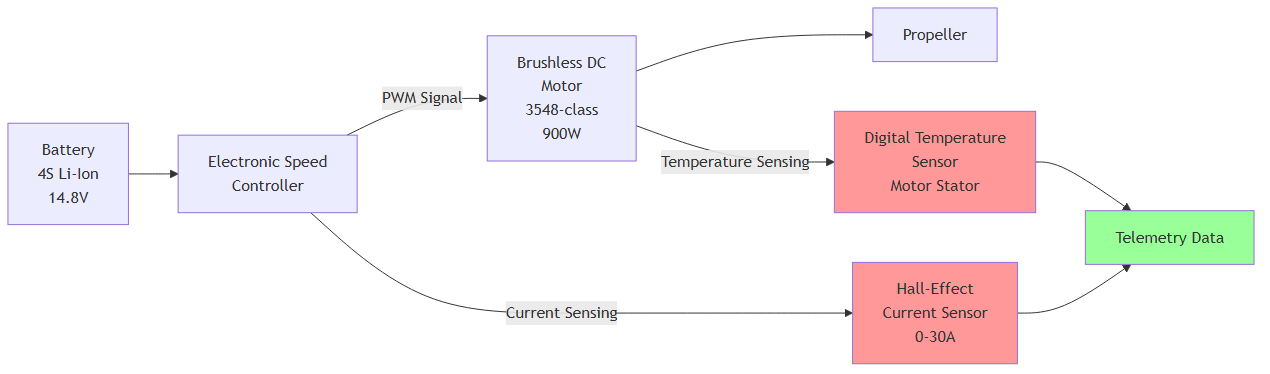
\includegraphics[width=0.9\textwidth]{assets/figures/chapter4/fig_propulsion_chain.png}
\fbox{\parbox[c][4cm][c]{0.6\textwidth}{\centering Figure: Propulsion chain diagram showing power flow and sensor placement}}
\caption{Propulsion chain diagram showing power flow and sensor placement.}
\label{fig:propulsion_chain}
\end{figure}

\subsection{Current Sensing Strategy}

A Hall-effect current sensor was selected for current measurement. Hall-effect sensors provide electrical isolation between the high-current power circuit and the low-voltage sensing circuit, which improves safety and signal quality. The sensor is placed on the ESC output to measure the total current delivered to the motor. The measurement range is selected as 0-30 Amperes to accommodate both nominal cruise current (approximately 10A) and degraded conditions (up to 20A or higher during bearing failure). The sensor resolution is selected as 0.1A to detect subtle current drift patterns indicative of early bearing wear. The sampling frequency is set to 10 Hz (10 samples per second), which is sufficient to detect gradual bearing wear while avoiding excessive data volume. This sampling frequency was selected because bearing wear is a slow mechanical process occurring over hours or days; high-frequency sampling would not provide additional predictive value for this failure mode. Alternative sensing technologies considered included shunt resistors with amplifiers, which were rejected due to lack of electrical isolation, and current transformers, which were rejected due to size and complexity.

\subsection{Temperature Sensing Strategy}

A digital temperature sensor placed on the motor stator was selected for temperature measurement. The stator is the stationary part of the motor where the copper windings are located, and it experiences the most significant temperature rise due to resistive heating (Ploss = I²R). Measuring stator temperature provides the most accurate indication of motor thermal stress. The sensor measurement range is selected as 0-100°C to cover nominal operating temperatures (near 50°C) and degraded conditions (up to 70°C or higher). The sensor accuracy is selected as ±1°C to detect subtle temperature drift patterns. The sampling frequency is synchronized with the current sensor at 10 Hz to ensure consistent time-series data. The physical relationship between current and temperature is governed by thermal dynamics: electrical heat generation in the stator coils is proportional to the square of the current (Ploss = I² × R). Therefore, as bearing wear increases friction, the motor draws more current to maintain speed, and the temperature rises exponentially. This physical relationship justifies monitoring both parameters: current provides the direct indication of mechanical load, while temperature provides the thermal consequence of that load.

\subsection{Telemetry Acquisition Chain}

The telemetry acquisition chain transforms physical sensor signals into digital time-series data suitable for machine learning analysis. The chain begins with the sensors (Hall-effect current sensor on ESC output, digital temperature sensor on motor stator). The sensor signals undergo signal conditioning, which includes amplification, filtering, and noise reduction to improve signal quality. The conditioned analog signals are converted to digital values through analog-to-digital conversion (ADC) at a sampling rate of 10 Hz. The digital values are transmitted to a microcontroller or flight computer, which packages the data with timestamps and stores it locally or transmits it to a ground station. For this project, the telemetry data is stored in CSV format for offline analysis and training of the machine learning model. The physics-based relationship underlying the telemetry is: as bearings wear out, mechanical friction increases; to overcome this friction and maintain constant cruise speed (5000 RPM), the ESC must supply more electrical current; according to thermal dynamics, electrical heat generation is proportional to the square of the current (Ploss = I²R); therefore, the motor temperature rises exponentially. This chain of physical phenomena generates the time-series patterns that the Isolation Forest algorithm detects as anomalies.

\begin{figure}[H]
\centering
% 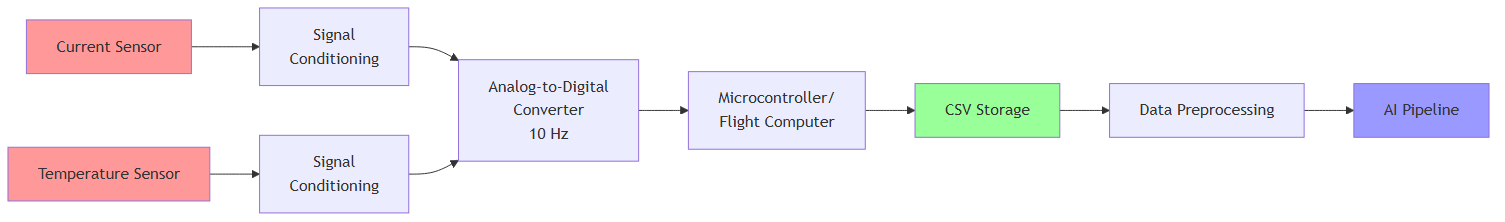
\includegraphics[width=0.9\textwidth]{assets/figures/chapter4/fig_telemetry_chain.png}
\fbox{\parbox[c][4cm][c]{0.6\textwidth}{\centering Figure: Telemetry acquisition chain from physical sensors to AI pipeline}}
\caption{Telemetry acquisition chain from physical sensors to AI pipeline.}
\label{fig:telemetry_chain}
\end{figure}

\subsection{Failure Mode Analysis}

Motor failure modes can be classified into two categories: instantaneous failures and progressive failures. Instantaneous failures include broken propeller blades, burnt ESC MOSFETs, disconnected wire phases, and demagnetised rotor magnets. These failures occur suddenly and without warning precursors, making them unsuitable for predictive maintenance. When a wire disconnects or the ESC blows up, the drone crashes immediately; these failures require reactive maintenance (fixing after they occur). Progressive failures include bearing wear, which occurs gradually over hours or days. Bearing wear happens slowly as the bearings lose lubrication, become scratched, and increase friction. This slow, creeping mechanical failure generates time-series data—a slowly rising current and a slowly rising temperature. This gradual deterioration is exactly the type of trend that predictive maintenance machine learning is designed to detect before catastrophic failure occurs. Among all motor failure modes, bearing wear was selected as the focus of this project because it is the only failure mode that: (1) is progressive rather than instantaneous, (2) generates measurable precursors (current and temperature drift), (3) occurs over a timescale suitable for early warning, and (4) represents a significant maintenance cost for UAV operators.

\begin{figure}[H]
\centering
% 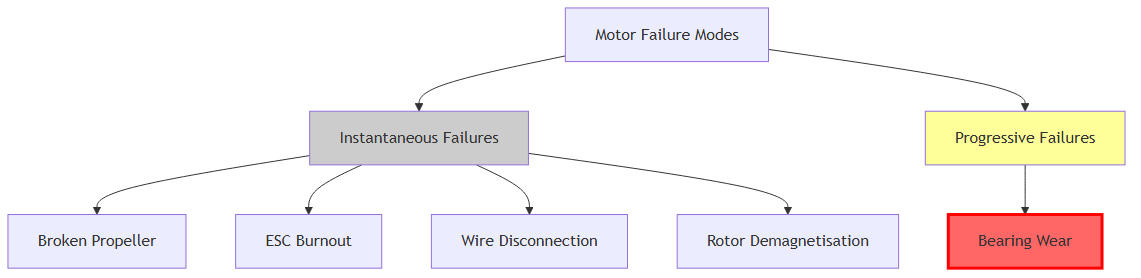
\includegraphics[width=0.7\textwidth]{assets/figures/chapter4/fig_failure_modes.png}
\fbox{\parbox[c][4cm][c]{0.6\textwidth}{\centering Figure: Failure mode classification tree highlighting bearing wear as the selected target}}
\caption{Failure mode classification tree highlighting bearing wear as the selected target.}
\label{fig:failure_modes}
\end{figure}

\subsection{Monitoring Parameter Justification}

The initial technical specification proposed monitoring five avionics-related parameters: electrical voltage levels, electrical current measurements, temperature sensor data, error rate counters, and communication message frequency. However, after discussion with the industrial supervisor, the project scope was focused specifically on the UAV propulsion system (brushless DC motor and ESC) with emphasis on bearing wear detection. Consequently, the monitoring scope was reduced to two parameters: motor current (Amperes) and motor temperature (degrees Celsius). This scope reduction is justified by several factors. First, current and temperature have a direct physical relationship through thermal dynamics (Ploss = I²R), making them highly correlated indicators of mechanical load. Second, bearing wear manifests as increased friction, which directly increases current draw and consequently temperature. Third, voltage monitoring was removed because voltage is primarily determined by battery state of charge rather than motor health. Fourth, error rate counters were removed because they are more relevant to communication systems than propulsion systems. Fifth, communication frequency was removed because it is not directly related to mechanical degradation. The focus on current and temperature provides sufficient information to detect bearing wear while maintaining system simplicity and reducing implementation complexity. This scope reduction aligns with the industrial supervisor's guidance to focus on the most critical component (the motor) and the most detectable failure mode (bearing wear).

\begin{figure}[H]
\centering
% 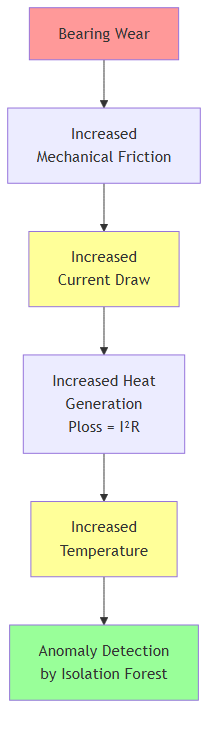
\includegraphics[width=0.9\textwidth]{assets/figures/chapter4/fig_current_temp_relationship.png}
\fbox{\parbox[c][4cm][c]{0.6\textwidth}{\centering Figure: Physical relationship between bearing wear, current, and temperature}}
\caption{Physical relationship between bearing wear, current, and temperature.}
\label{fig:current_temp_relationship}
\end{figure}

\section{Software Architecture}

\subsection{Global Software Architecture}

The software architecture follows a layered architecture pattern, which provides clear separation of concerns and facilitates modular development. The system is composed of five main components: the Streamlit Dashboard (frontend), the FastAPI Backend (API layer), the AI Engine (Isolation Forest), the SQLite Database (data persistence), and the Authentication component (security). The layered architecture organizes these components into four layers: the presentation layer (Streamlit Dashboard), the application layer (FastAPI Backend), the business logic layer (AI Engine), and the data layer (SQLite Database). The Authentication component spans the presentation and application layers to secure access. This architecture was selected over alternatives such as microservices architecture because it is simpler to implement for a single-developer Final Year Project while still providing sufficient modularity for future expansion. The system boundaries are clearly defined: the Dashboard communicates only with the Backend API, the Backend API communicates with the Database and AI Engine, and the AI Engine operates independently with data persistence through the Database. This separation enables independent development and testing of each component.

\begin{figure}[H]
\centering
% 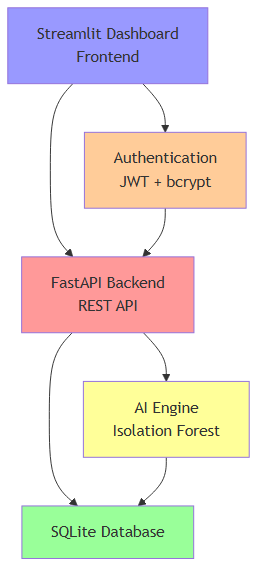
\includegraphics[width=0.9\textwidth]{assets/figures/chapter4/fig_global_architecture.png}
\fbox{\parbox[c][4cm][c]{0.6\textwidth}{\centering Figure: Global software architecture showing five main components}}
\caption{Global software architecture showing five main components.}
\label{fig:global_architecture}
\end{figure}

\begin{figure}[H]
\centering
% 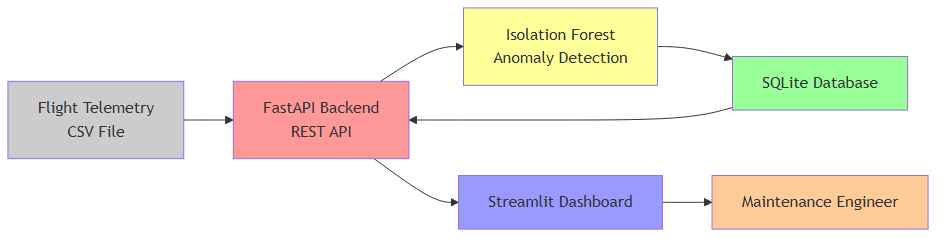
\includegraphics[width=0.9\textwidth]{assets/figures/chapter4/fig_system_dataflow.png}
\fbox{\parbox[c][4cm][c]{0.6\textwidth}{\centering Figure: System dataflow from telemetry ingestion to maintenance engineer visualization}}
\caption{System dataflow from telemetry ingestion to maintenance engineer visualization.}
\label{fig:system_dataflow}
\end{figure}

\subsection{Component Architecture}

The component architecture defines the responsibilities and interactions of each system component. The Streamlit Dashboard component is responsible for user interface rendering, real-time data visualization, and user interaction handling. It communicates with the FastAPI Backend through HTTP requests using a polling approach (the dashboard periodically queries the API for updated data). The FastAPI Backend component is responsible for request handling, business logic coordination, and data access. It exposes REST API endpoints for authentication, flight data retrieval, and anomaly queries. The AI Engine component is responsible for data preprocessing, model training, model inference, and anomaly detection. It operates as a separate module that can be invoked by the Backend or run independently for batch processing. The SQLite Database component is responsible for persistent storage of user accounts, flight sessions, telemetry readings, and anomaly events. The Authentication component is responsible for user login, JWT token generation, token validation, and role-based access control enforcement. Components interact through well-defined interfaces: the Dashboard calls API endpoints, the API queries the Database and invokes the AI Engine, and the AI Engine reads from and writes to the Database.

\begin{figure}[H]
\centering
% 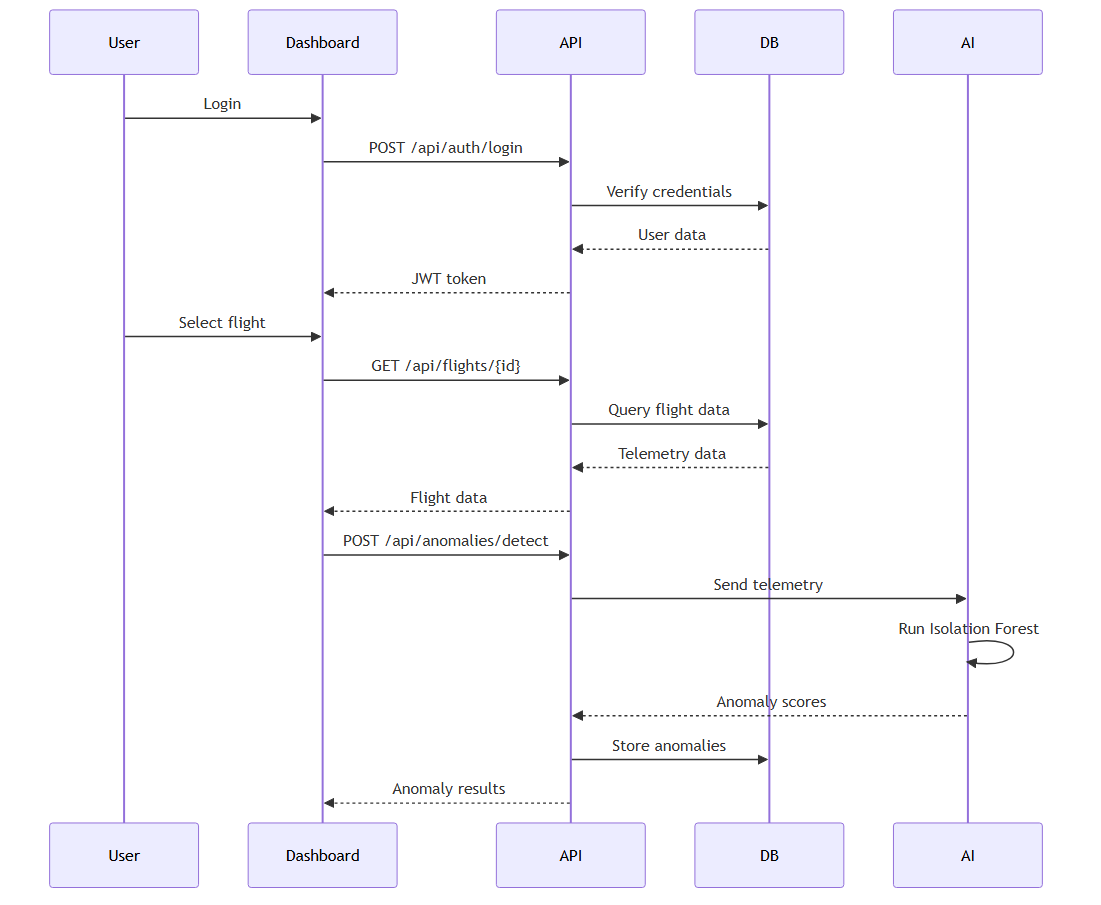
\includegraphics[width=0.9\textwidth]{assets/figures/chapter4/fig_component_interaction.png}
\fbox{\parbox[c][4cm][c]{0.6\textwidth}{\centering Figure: Component interaction sequence diagram}}
\caption{Component interaction sequence diagram.}
\label{fig:component_interaction}
\end{figure}

\subsection{Frontend Architecture}

The frontend architecture is based on the Streamlit framework, which was selected over alternatives such as React.js for several reasons. Streamlit is specifically designed for data applications and machine learning dashboards, making it ideal for this project's focus on telemetry visualization and anomaly detection. Streamlit provides built-in components for charts, graphs, and data tables, which accelerates development compared to building custom components in React.js. Streamlit's Python-based approach eliminates the need for JavaScript development, reducing the technology stack complexity for a single-developer project. The Dashboard page structure is organized into three main views: the authentication view (login form), the monitoring view (real-time telemetry charts and health status), and the historical view (past flight data and anomaly analysis). Real-time data visualization is implemented through a polling approach: the dashboard queries the Backend API every 5 seconds for updated telemetry data, which is sufficient for bearing wear monitoring given the slow degradation rate. User interface components include line charts for current and temperature trends, status indicators for health scores, alert panels for anomaly notifications, and flight selectors for historical data access. State management in Streamlit is handled through session state, which maintains user authentication status and selected flight context across page interactions.

\subsection{Backend Architecture}

The backend architecture is based on the FastAPI framework, which was selected for its performance, automatic API documentation, and native support for asynchronous operations. FastAPI provides a modern Python web framework that is faster than alternatives such as Flask while being simpler than Django for API-only applications. The API endpoint organization follows RESTful principles: authentication endpoints (/api/auth/login, /api/auth/logout), user management endpoints (/api/users), flight data endpoints (/api/flights, /api/flights/{id}, /api/flights/{id}/telemetry), and anomaly endpoints (/api/anomalies, /api/anomalies/{id}). Request and response handling uses JSON format for data exchange. The business logic layer coordinates between API endpoints and the data access layer, implementing validation logic and business rules. The data access layer uses SQLAlchemy ORM to interact with the SQLite Database, providing an abstraction layer that simplifies database operations and enables future migration to PostgreSQL if needed. The backend architecture is designed to be stateless, with all state managed through the Database and JWT tokens, which facilitates horizontal scaling if required in future production deployments.

\subsection{AI Pipeline Architecture}

The AI pipeline architecture defines the flow of data from raw telemetry to anomaly detection results. The pipeline consists of five stages: data ingestion, data preprocessing, model training, model inference, and anomaly storage. Data ingestion reads telemetry data from CSV files and inserts it into the SQLite Database through the TelemetryReading table. Data preprocessing performs data cleaning (removing null values, filtering outliers), normalization (scaling current and temperature to standard ranges), and feature engineering (computing rolling averages to smooth noise). Model training loads healthy flight data (flights without bearing degradation), trains an Isolation Forest model with a contamination parameter tuned to the expected anomaly rate, and saves the trained model to disk as a pickle file. Model inference loads the trained model, processes new telemetry data through the same preprocessing pipeline, applies the model to generate anomaly scores, and classifies data points as normal or anomalous based on a threshold. Anomaly storage writes detected anomalies to the AnomalyEvent table in the Database with associated metadata (timestamp, severity, description). The AI pipeline is designed to be modular: each stage can be run independently (e.g., model training can be performed offline, while inference runs in real-time). Model persistence uses pickle file storage, which is simple and sufficient for the prototype scope; future production deployments could use MLflow or similar model management systems.

\begin{figure}[H]
\centering
% 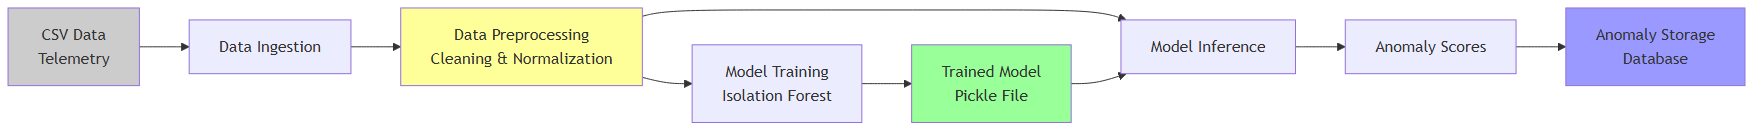
\includegraphics[width=0.9\textwidth]{assets/figures/chapter4/fig_ai_pipeline.png}
\fbox{\parbox[c][4cm][c]{0.6\textwidth}{\centering Figure: AI pipeline architecture from data ingestion to anomaly storage}}
\caption{AI pipeline architecture from data ingestion to anomaly storage.}
\label{fig:ai_pipeline}
\end{figure}

\subsection{Database Architecture}

The database architecture uses SQLite as the database management system. SQLite was selected over alternatives such as PostgreSQL for several reasons: SQLite requires no server setup or configuration, which simplifies deployment for a prototype; SQLite stores data in a single file, which facilitates backup and portability; SQLite provides sufficient performance for the expected data volume (hundreds of flights with thousands of telemetry points); SQLite supports the full SQL standard and SQLAlchemy ORM, enabling future migration to PostgreSQL if needed. The database schema consists of four main tables: User, FlightSession, TelemetryReading, and AnomalyEvent. The User table stores user account information including username, email, password hash, and role (Administrator, Maintenance Engineer, Drone Operator). The FlightSession table stores flight metadata including session ID, associated user ID, start timestamp, end timestamp, and flight status. The TelemetryReading table stores time-series telemetry data including reading ID, associated flight session ID, timestamp, current value, temperature value, and RPM value. The AnomalyEvent table stores detected anomalies including event ID, associated flight session ID, timestamp, anomaly type, severity level, and description. Relationships between tables are enforced through foreign keys: FlightSession references User, TelemetryReading references FlightSession, and AnomalyEvent references FlightSession. Data volume estimation for the prototype assumes approximately 100 flights with 3600 telemetry points per flight (1 hour at 1 Hz sampling), resulting in approximately 360,000 telemetry readings, which SQLite can handle efficiently. Database migrations are managed using Alembic, which provides version control for schema changes and enables rollback if needed.

\begin{figure}[H]
\centering
% 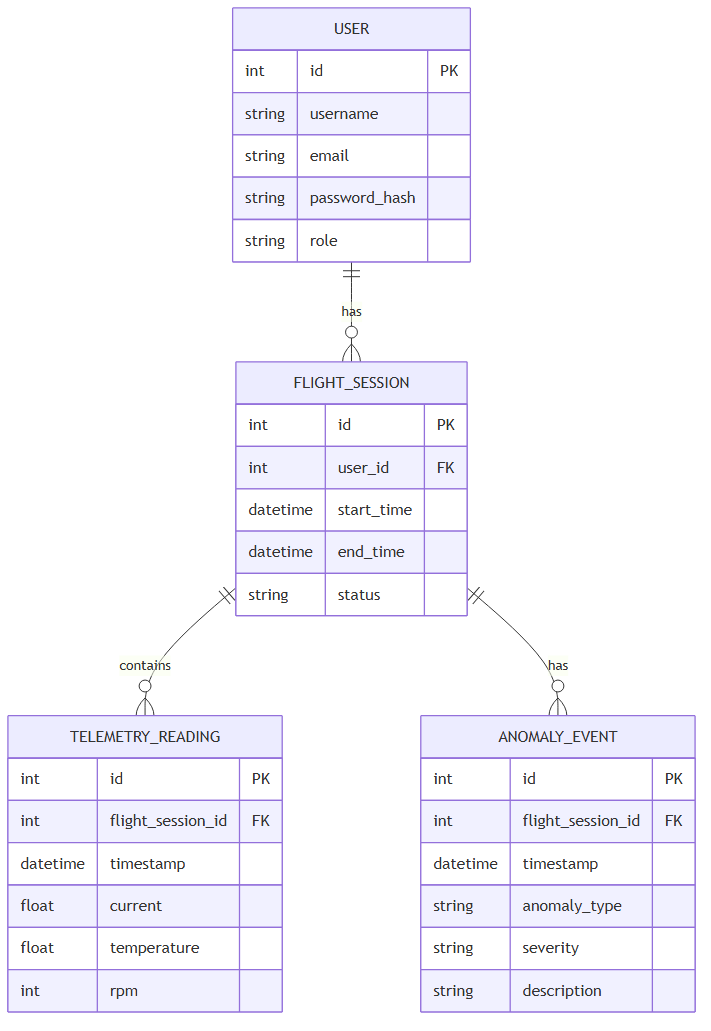
\includegraphics[width=0.9\textwidth]{assets/figures/chapter4/fig_database_schema.png}
\fbox{\parbox[c][4cm][c]{0.6\textwidth}{\centering Figure: Database schema (ER diagram) showing four main tables and relationships}}
\caption{Database schema (ER diagram) showing four main tables and relationships.}
\label{fig:database_schema}
\end{figure}

\subsection{Authentication and Authorization Strategy}

The authentication strategy is based on JSON Web Tokens (JWT). JWT was selected over session-based authentication because it is stateless, which aligns with the RESTful API architecture and simplifies scalability. The authentication flow begins when a user submits their username and password through the Dashboard login form. The Backend verifies the credentials by comparing the password hash (stored using bcrypt, a secure hashing algorithm) with the hash of the submitted password. If credentials are valid, the Backend generates a JWT token containing the user ID and role, signs it with a secret key, and returns it to the Dashboard. The Dashboard stores the token and includes it in the Authorization header of subsequent API requests. The Backend validates the token on each request by verifying the signature and checking the expiration time (set to 24 hours). Authorization is implemented through role-based access control (RBAC). Three roles are defined: Administrator (full system access including user management), Maintenance Engineer (access to monitoring, historical data, and anomaly analysis), and Drone Operator (access to real-time alerts and basic status only). The Backend enforces RBAC by checking the user's role in the JWT token and denying access to endpoints that require higher privileges. Session management is handled through JWT expiration; when a token expires, the user must re-authenticate. Security considerations include: password hashing with bcrypt to prevent credential theft if the database is compromised; JWT token expiration to limit the window of token misuse; HTTPS encryption for all API communications in production deployments; and input validation to prevent SQL injection and other injection attacks.

\begin{figure}[H]
\centering
% 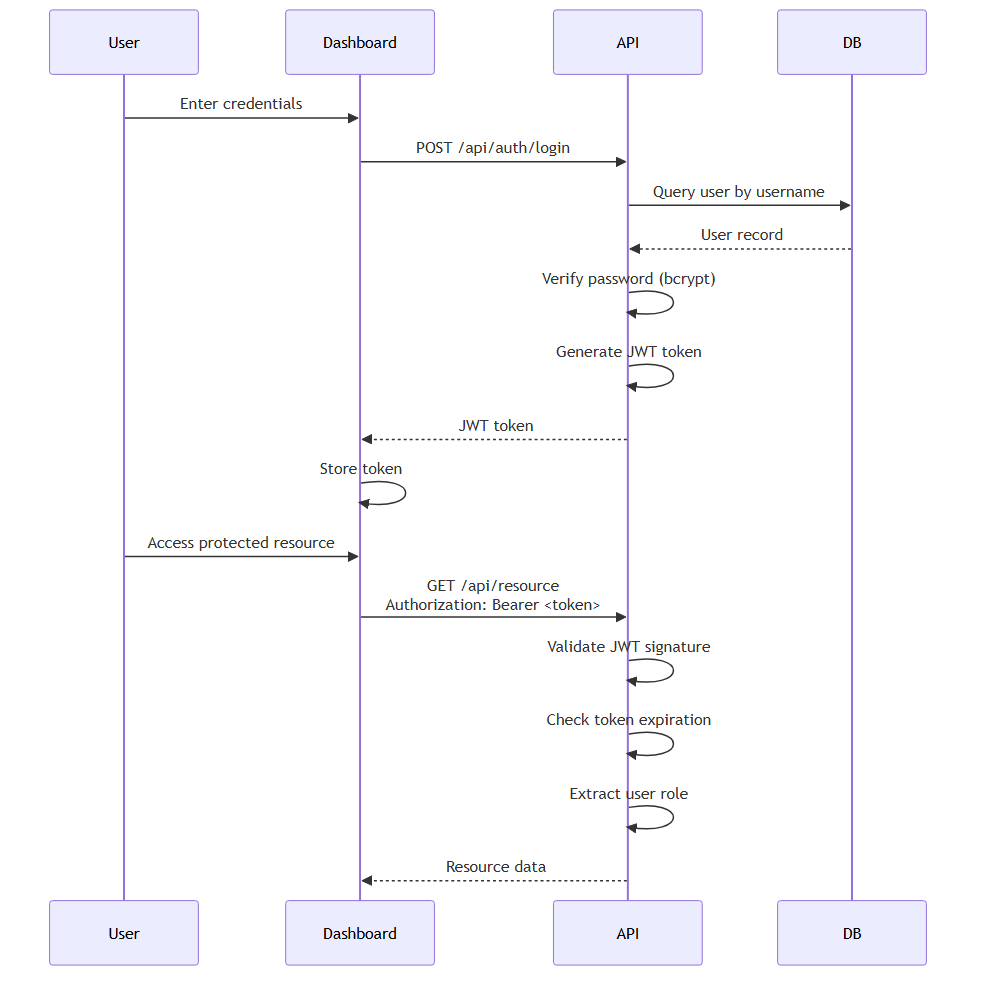
\includegraphics[width=0.9\textwidth]{assets/figures/chapter4/fig_auth_flow.png}
\fbox{\parbox[c][4cm][c]{0.6\textwidth}{\centering Figure: Authentication flow diagram showing JWT-based login and API access}}
\caption{Authentication flow diagram showing JWT-based login and API access.}
\label{fig:auth_flow}
\end{figure}

\subsection{Deployment Architecture}

The deployment architecture targets a local development environment or single-server deployment for the prototype phase. All components (Dashboard, Backend, AI Engine, Database) are deployed on a single machine, which simplifies development and testing. The Dashboard runs as a Streamlit application on a configurable port (default 8501). The Backend runs as a FastAPI application on a configurable port (default 8000). The Database is stored as a SQLite file in the project directory. The AI Engine operates as a Python module that can be invoked by the Backend or run as a standalone script. Environment configuration is managed through environment variables or a configuration file, which stores settings such as database file path, JWT secret key, API port, and Dashboard port. Data persistence is ensured through the SQLite file, which survives application restarts. Scalability considerations for the prototype are limited: SQLite has concurrency limitations that may become problematic with multiple simultaneous users, but this is acceptable for the single-user or few-user prototype scope. Future production deployments would require several architectural changes: migration from SQLite to PostgreSQL for better concurrency and data volume handling; deployment of components on separate servers or containers for improved performance and fault tolerance; implementation of load balancing for the Backend API; and addition of monitoring and logging infrastructure for operational visibility. However, these production concerns are outside the scope of the current prototype, which focuses on demonstrating the feasibility of predictive maintenance for UAV propulsion systems.

\begin{figure}[H]
\centering
% 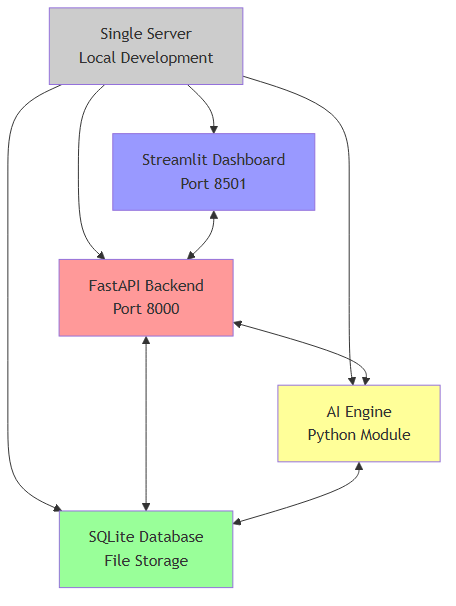
\includegraphics[width=0.8\textwidth]{assets/figures/chapter4/fig_deployment.png}
\fbox{\parbox[c][4cm][c]{0.6\textwidth}{\centering Figure: Deployment architecture showing single-machine prototype configuration}}
\caption{Deployment architecture showing single-machine prototype configuration.}
\label{fig:deployment}
\end{figure}

\subsection{Technology Stack Justification}

The technology stack selection balances simplicity, performance, and suitability for the project scope. Python was selected as the primary programming language because it provides excellent support for data science (Pandas, NumPy), machine learning (Scikit-learn), and web development (FastAPI, Streamlit), reducing the need to learn multiple languages. FastAPI was selected as the backend framework over alternatives such as Flask and Django because it provides better performance through asynchronous support, automatic API documentation (Swagger UI), and native data validation through Pydantic. Flask was rejected because it requires more boilerplate code for API development. Django was rejected because it is designed for full-stack web applications with built-in ORM and templating, which adds unnecessary complexity for an API-only backend. Streamlit was selected as the frontend framework over React.js because it is specifically designed for data applications, provides built-in visualization components, and eliminates the need for JavaScript development. React.js was rejected because it would require additional frontend development effort and technology stack complexity. SQLite was selected as the database over PostgreSQL because it requires no server setup, simplifies deployment, and provides sufficient performance for the prototype data volume. PostgreSQL was rejected because it requires server configuration and adds deployment complexity, though it remains a viable option for future production migrations. Scikit-learn was selected as the machine learning library because it provides a well-documented implementation of Isolation Forest, is widely used in academia and industry, and integrates seamlessly with the Python data science ecosystem. Pandas was selected for data manipulation because it provides efficient data structures for time-series data and integrates with Scikit-learn for machine learning workflows. Alternative technology stacks considered included a JavaScript-based stack (Node.js + React) and a Java-based stack (Spring Boot + Angular), but these were rejected due to weaker machine learning library support and increased complexity for a single-developer project.

\section*{Conclusion to Chapter 4}
\addcontentsline{toc}{section}{Conclusion to Chapter 4}

This chapter has presented the design and architecture of the Intelligent Avionics Health Monitoring and Predictive Maintenance Platform. The UAV conceptual design established the physical baseline: a fixed-wing Blended Wing Body UAV with a rear-mounted pusher propulsion system, focusing on brushless DC motor bearing wear as the target failure mode. The sensing strategy was defined with Hall-effect current sensing on the ESC output and digital temperature sensing on the motor stator, both sampled at 10 Hz. The monitoring scope was justified to focus on current and temperature parameters, which have a direct physical relationship through thermal dynamics and provide sufficient information for bearing wear detection. The software architecture was designed as a layered architecture with five main components: Streamlit Dashboard, FastAPI Backend, AI Engine, SQLite Database, and Authentication. The component architecture defined clear responsibilities and interactions for each component. The frontend architecture leverages Streamlit for rapid development of data visualization interfaces. The backend architecture uses FastAPI for high-performance REST API endpoints. The AI pipeline architecture defines the flow from data ingestion to anomaly detection. The database architecture uses SQLite with four tables for persistent storage. The authentication strategy uses JWT with bcrypt for secure access control. The deployment architecture targets a single-machine prototype with clear paths to production scaling. The technology stack was justified by balancing simplicity, performance, and suitability for the project scope. The design decisions presented in this chapter establish the foundation for the implementation phases described in the subsequent chapters. The next chapter will present Sprint 0, which covers the initialization phase including scope finalization, UAV context documentation, and detailed software architecture design.
